% CSC-44102 Assessment 1 report.
%
% Black and white only: no colour packages; links are not coloured.
% Text marked [YOUR WORDS: ...] must be written by the author before
% submission; the PDF shows these markers in bold so none is missed.

\documentclass[11pt,a4paper]{article}

\usepackage[british]{babel}  % British spelling and date format
\usepackage[T1]{fontenc}
\usepackage[utf8]{inputenc}
\usepackage[margin=2.5cm]{geometry}
\usepackage{lmodern}
\usepackage{graphicx}       % \includegraphics for screenshots
\usepackage{booktabs}       % clean black-and-white tables
\usepackage{tabularx}       % tables with wrapping columns
\usepackage{listings}       % code excerpts, monochrome (set-up below)
\usepackage{csquotes}
\usepackage{tikz}           % diagrams, black and white
\usetikzlibrary{arrows.meta,calc,positioning}

% Referencing: author-year style.
% useprefix keeps name prefixes: "van Rossum", not "Rossum".
\usepackage[backend=biber,style=authoryear,useprefix=true]{biblatex}
\addbibresource{references.bib}

\usepackage[hidelinks]{hyperref}  % load last; hidelinks keeps links black

\lstset{
  basicstyle=\ttfamily\small,
  frame=single,
  breaklines=true,
  columns=fullflexible,
  keepspaces=true,
  numbers=left,
  numberstyle=\tiny,
  showstringspaces=false
}

% Screenshots: the repository's docs/screenshots folder, or a screenshots
% folder next to this file when the report is compiled on its own.
\graphicspath{{../docs/screenshots/}{screenshots/}}

\newcommand{\yourwords}[1]{\textbf{[YOUR WORDS: #1]}}
\newcommand{\code}[1]{\texttt{#1}}

\begin{document}

% Front matter numbered i, ii, ...; the report itself from 1. Without this the
% title page and the first section are both "page 1", which breaks PDF links.
\pagenumbering{roman}
\hypersetup{pageanchor=false}  % the title page gets no PDF page anchor

\begin{titlepage}
  \centering
  {\Large CSC-44102 Foundations of Programming and Software Engineering\par}
  \vspace{1em}
  {\Large Assessment 1: Technical Report\par}
  \vspace{2em}
  {\LARGE Study Planner: a task and deadline manager\\
  in two versions over one shared core\par}
  \vfill
  [Full name]\par
  [Student number]\par
  \vspace{1em}
  Word count: [number]\par
  \vspace{1em}
  [Submission date]\par
\end{titlepage}
\hypersetup{pageanchor=true}


\section*{Abstract}
\addcontentsline{toc}{section}{Abstract}
Students juggle coursework tasks from several modules, each with its own
deadline and priority. This report describes the Study Planner, a Python
application that records study tasks, tracks their progress and shows what
is overdue. It has a text-based version and a Tkinter graphical version with
the same functionality, both built on one shared core module that holds all
validation, task rules, search, filtering, a stable merge sort, the progress
summary and safe JSON storage. Eleven functional and nine non-functional
requirements, prioritised with MoSCoW, define the application through 77
testable acceptance criteria. A test plan of 304 cases (normal, boundary and
invalid) is implemented as 317 automated tests, all of which pass; branch
coverage of the source code is 97\%. The evaluation finds every requirement
met and discusses the remaining limitations.

\clearpage
\tableofcontents
\clearpage
\pagenumbering{arabic}

% ---------------------------------------------------------------------------
\section{Introduction}

\subsection{Problem}
A student's coursework arrives from several modules at once: essays, lab
reports, revision and problem sheets, each with a due date. Keeping these in
memory or in scattered notes makes it easy to miss a deadline or to lose
track of what is already finished. A small, reliable tool that keeps every
task in one place, with its subject, priority, status and due date, and that
shows overall progress, addresses this problem.

\subsection{Aims and objectives}
The aim is a Study Planner that a student can use from the command line or
from a window, with the same behaviour in both. The objectives are:
\begin{enumerate}
  \item add, edit and delete study tasks, and change their status;
  \item validate every input and reject invalid data with clear messages;
  \item save tasks to a local file automatically and load them at start-up,
        without ever losing or corrupting data;
  \item search, filter and sort the task list;
  \item summarise progress: total, completed, remaining and overdue tasks and
        the completion percentage;
  \item provide a text-based and a Tkinter version that share one core
        module, so neither interface implements business rules;
  \item test every requirement with automated tests.
\end{enumerate}

\subsection{Scope}
The application records, for each task, a title, a subject, an optional
description, a due date, a priority (High, Medium, Low) and a status
(Pending, In Progress, Completed). It is a single-user, local application.
User accounts, cloud synchronisation and a database are out of scope.

% ---------------------------------------------------------------------------
\section{Requirements}

Each requirement is numbered, has a priority and is defined by acceptance
criteria (ACs) of the form \enquote{given \ldots, when \ldots, the application
shall \ldots}, with exact inputs and expected results, so that every
criterion can be tested. Priorities use MoSCoW: \emph{Must} for what a working
application needs to meet the brief's Pass guide, \emph{Should} for important
planned features without which the application would still meet that guide,
\emph{Could} for features to drop first if time ran short, and \emph{Won't}
for deliberate exclusions. All Must, Should and Could requirements were
implemented.

\subsection{Functional requirements}

\begin{table}[ht]
\centering
\small
\begin{tabularx}{\textwidth}{@{}llcX@{}}
\toprule
ID & Requirement & Priority & Summary and justification \\
\midrule
FR1 & Add task & Must & New task with the next unused ID, defaults Medium and Pending. Everything else depends on adding tasks. \\
FR2 & Edit task & Should & Change title, subject, description, due date or priority; all or nothing. Useful, but deletion already removes mistakes. \\
FR3 & Delete task & Must & Remove one task after confirmation; IDs are never reused. \\
FR4 & Change status & Must & The only way to change a status. Progress tracking is the purpose of the topic. \\
FR5 & Input validation & Must & One set of rules in the core; all errors reported together. Required by the Pass guide. \\
FR6 & Persistence & Must & Strict JSON loading, safe saving, unsaved-change handling. The Pass guide requires file reading and writing. \\
FR7 & Search & Should & Case-insensitive partial match in title, description and subject. Sorting already supplies the algorithm. \\
FR8 & Filter & Could & Status, priority and subject filters combined with AND. Overlaps with search. \\
FR9 & Sort & Must & By due date, priority, status or subject with a stable merge sort: the required non-trivial algorithm. \\
FR10 & Summary & Should & Total, completed, remaining, overdue and completion percentage. Central to the topic but not a Pass minimum. \\
FR11 & View task list & Must & The list in stored order, or as search, filters and sort specify. \enquote{View} is a Pass-guide feature. \\
\bottomrule
\end{tabularx}
\caption{Functional requirements with MoSCoW priorities.}
\label{tab:fr}
\end{table}

The requirements specification gives each requirement in full with its
77 acceptance criteria. Two examples show the level of detail. FR5 fixes the
exact error for every field and rule, for example
\enquote{Due date must be a real calendar date.} for \code{2026-02-30}, and
the order in which several errors are reported. FR9 AC5 requires the subject
sort to use \code{casefold()}: with the stored subject \code{biology}, the
order must be tasks 5, 3, 2, 4, 1, whereas a plain string comparison would
wrongly give 5, 2, 4, 1, 3.

\subsection{Non-functional requirements}

\begin{table}[ht]
\centering
\small
\begin{tabularx}{\textwidth}{@{}llcX@{}}
\toprule
ID & Requirement & Priority & Measure \\
\midrule
NFR1 & Usability and feedback & Should & Feedback matches the exact messages specified by FR1--FR11 in both versions. \\
NFR2 & Code quality & Must & Code compiles; \code{pycodestyle} reports zero PEP~8 \parencite{pep8} errors; both interfaces use the shared core. \\
NFR3 & Reliability & Must & No unhandled exception on any tested invalid input; failed saves lose no data; invalid files are never overwritten. \\
NFR4 & Input validation & Must & FR5 is the single source of validation; one invalid input per interface goes through the core. \\
NFR5 & Portability & Must & Python 3.12, standard library and Tkinter only; runs in a fresh virtual environment. \\
NFR6 & Performance & Could & Search and sort times measured on 500 tasks. \\
NFR7 & Test traceability & Should & Every AC maps to at least one test with a recorded result; coverage measured. \\
NFR8 & Data storage & Should & Data in \code{\textasciitilde/.study\_planner/tasks.json}; tests use temporary folders only. \\
NFR9 & Documentation & Must & Instructions for running both versions and the tests, reproducible from a fresh copy. \\
\bottomrule
\end{tabularx}
\caption{Non-functional requirements with MoSCoW priorities.}
\label{tab:nfr}
\end{table}

NFR6 is deliberately a \emph{Could}: a personal planner rarely holds more than
a few hundred tasks, so the requirement asks for a measurement, and a numeric
threshold is set only after measuring. \yourwords{state the NFR6 threshold you
choose now that the measurements in Section~\ref{sec:testing} exist, or
explain why the requirement stays a measurement only.}

% ---------------------------------------------------------------------------
\section{Design}

\subsection{Program structure}
The application has four modules (Figure~\ref{fig:modules}). \code{core.py}
holds every business rule: validation, the task operations, search, filters,
the merge sort, the summary and the message table. \code{storage.py} only
loads and saves the JSON file. \code{cli.py} and \code{gui.py} only collect
input and display results. Only the core calls the storage module, so both
interfaces reach the file through the same save, retry and unsaved-state
logic. Because the interfaces contain no rules, the GUI was added as a new
front end without changing the behaviour of the core.

\begin{figure}[ht]
\centering
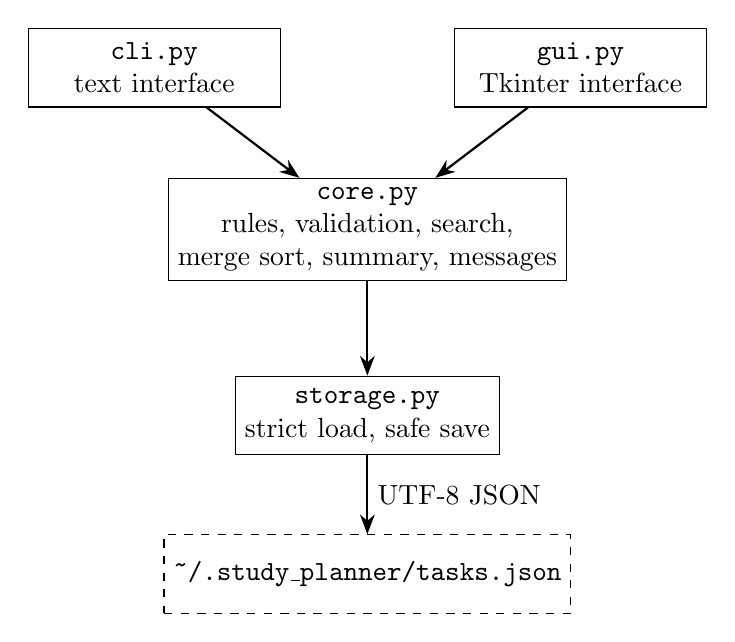
\begin{tikzpicture}[
    box/.style={draw, rectangle, minimum width=3.2cm, minimum height=1cm,
                align=center},
    arrow/.style={-{Stealth[length=2.5mm]}, thick}]
  \node[box] (cli) {\code{cli.py}\\text interface};
  \node[box, right=2.2cm of cli] (gui) {\code{gui.py}\\Tkinter interface};
  \node[box, below=1.4cm of $(cli)!0.5!(gui)$] (core)
    {\code{core.py}\\rules, validation, search,\\merge sort, summary, messages};
  \node[box, below=1.2cm of core] (storage)
    {\code{storage.py}\\strict load, safe save};
  \node[box, dashed, below=1.0cm of storage] (file)
    {\code{\textasciitilde/.study\_planner/tasks.json}};
  \draw[arrow] (cli) -- (core);
  \draw[arrow] (gui) -- (core);
  \draw[arrow] (core) -- (storage);
  \draw[arrow] (storage) -- node[right] {UTF-8 JSON} (file);
\end{tikzpicture}
\caption{Module structure. Arrows show which module calls which; the
interfaces never call the storage module.}
\label{fig:modules}
\end{figure}

\subsection{Data structures}
\begin{itemize}
  \item \textbf{List of task dictionaries.} The tasks are kept in a Python
        list in stored order; each task is a dictionary with the keys
        \code{id}, \code{title}, \code{subject}, \code{description},
        \code{due\_date}, \code{priority} and \code{status}. A list preserves
        the order required by FR11 (new tasks are appended, edited tasks keep
        their position) and maps directly to and from JSON.
  \item \textbf{ID counter.} \code{next\_id} is stored with the tasks, so an ID
        is never reused after a deletion (FR3 AC5).
  \item \textbf{Dictionaries as lookup tables.} The central message table maps
        message keys to templates, so both interfaces show the same text, and
        rank tables map priorities and statuses to their sort order.
  \item \textbf{Session view state.} A small data class holds the search query,
        the three filters and the selected sort. It is kept apart from the
        task data, so it is never saved and resets on restart (FR7--FR9).
  \item \textbf{Result objects.} Every operation returns an immutable result
        carrying the outcome (success, no change, invalid, not found), the
        message key and its parameters, and whether saving succeeded. This
        separates \enquote{the edit worked} from \enquote{the file could not be
        written}, which the unsaved-state behaviour of FR6 depends on.
\end{itemize}

\subsection{Algorithms}
\paragraph{Search and filters.} One linear pass over the list keeps each task
that matches the search query (a case-folded substring test on three fields)
and every active filter. This takes $O(n)$ tests for $n$ tasks, which is
appropriate for a few hundred tasks.

\paragraph{Stable merge sort.} Sorting uses the application's own merge sort
rather than Python's \code{sorted()} (Figure~\ref{fig:pipeline}). Each task's
key is computed once in a linear pass, for example
\code{(priority rank, due date)} or \code{(subject.casefold(), due date)},
and the merge sort then compares only keys. When two keys are equal, the merge
takes the element from the left half first, so tasks with equal keys keep
their stored order: the sort is stable, which FR9 requires as the final
tie-breaker. The sort makes $O(n \log n)$ comparisons, uses $O(n)$ extra space,
and returns a new list, so the stored order is never changed. Its output is
checked against \code{sorted()} with the same keys on 200 random tasks.

\begin{figure}[ht]
\centering
\begin{tikzpicture}[
    step/.style={draw, rectangle, minimum height=1cm, align=center,
                 text width=2.6cm},
    arrow/.style={-{Stealth[length=2.5mm]}, thick}]
  \node[step] (tasks) {stored tasks\\(stored order)};
  \node[step, right=0.7cm of tasks] (pass) {linear pass:\\search AND filters};
  \node[step, right=0.7cm of pass] (keys) {compute each\\key once};
  \node[step, right=0.7cm of keys] (sort) {stable merge sort\\(new list)};
  \draw[arrow] (tasks) -- (pass);
  \draw[arrow] (pass) -- (keys);
  \draw[arrow] (keys) -- (sort);
\end{tikzpicture}
\caption{How a list view is produced. Without a selected sort, the filtered
tasks are shown in stored order.}
\label{fig:pipeline}
\end{figure}

\paragraph{Validation and the summary.} Validation trims each value, checks
the exact \code{YYYY-MM-DD} shape before the calendar date, and matches
priorities and statuses case-insensitively before storing their canonical
form. The summary counts overdue tasks against a date passed in by the
interface (the core never reads the clock, so tests can fix the date) and
rounds the completion percentage half-up with \code{Decimal}
\parencite{python-decimal}, so 1 of 16
tasks gives 6.3\% rather than the 6.2\% of default float formatting.

\subsection{Safe storage}
The file is UTF-8 JSON \parencite{python-json}. Loading is strict: a file
that breaks any rule, such as a duplicate key, a
non-canonical priority or a \code{next\_id} not greater than every ID, is
rejected as a whole and never modified. Saving writes the complete data to a
temporary file in the same folder, flushes it to disk and then replaces the
real file in one step with \code{os.replace} \parencite{python-os}, so an
interrupted save cannot
leave a half-written file. If a save fails, the change stays in memory and the
data is marked unsaved until the next successful save.

\subsection{Interface design}
Both versions show the same data and the same messages from the core.
\begin{itemize}
  \item \textbf{Text version.} A numbered menu offers view, add, edit, delete,
        change status, search, filter, sort and summary. The task list is a
        fixed-width table (ID, title, due date, priority, status) with long
        titles wrapped inside their column and the subject and description
        on indented lines beneath each task. The current search, filters and
        sort are shown above the table. While changes are unsaved, the menu
        shows \enquote{Unsaved changes}.
  \item \textbf{GUI version.} One window holds the search field, the filter
        drop-downs, a subject filter with its own clear button, the
        \enquote{Sort by} control, the task list, the action buttons and the
        summary panel (Figure~\ref{fig:gui}). Drop-downs offer only permitted
        values, so invalid priorities and statuses cannot be typed. Forms keep
        the entered values and show validation errors inside the form. The
        window title shows \enquote{(unsaved)} after a failed save.
\end{itemize}
The table layout of the text version follows design decision D9: fixed
column widths, titles wrapped with \code{textwrap}
\parencite{python-textwrap} and indented secondary lines, keeping every
line within 80 characters. \yourwords{the rationale for D9 in your own words:
why fixed columns with wrapped titles and indented subject and description
lines were chosen over truncating titles, a wide description column or
free-form lines.}

% ---------------------------------------------------------------------------
\section{Implementation}

\subsection{Shared core and storage}
\code{core.py} (about 850 lines) implements validation as one function per
operation context: adding applies the defaults Medium and Pending, editing
applies the same rules without defaults, and a status change requires a
status. The \code{Planner} class holds the tasks, \code{next\_id}, the unsaved
flag and the view state, and offers \code{add\_task}, \code{edit\_task},
\code{delete\_task}, \code{change\_status}, \code{list\_view} and
\code{summary}. Every operation checks a typed task ID, and that the task
exists, before asking for anything else, and saves automatically after a real
change; a no-op edit or status change saves nothing. \code{storage.py}
(about 160 lines) contains the strict loader and the safe saver described in
Section~3.

\subsection{Text-based version}
\code{cli.py} runs a menu loop that reads answers through an injectable
\code{read} function and prints through an injectable \code{write} function,
which lets the tests drive it with scripted input. Each menu action collects
the answers, passes them to the core and prints the result's lines. Deletion
asks for confirmation (only \code{y} or \code{yes} confirms). Exiting with
unsaved changes offers Retry saving, Exit without saving and Cancel exit.
Unexpected errors are logged to standard error, without task content, and the
user sees a short message instead of a traceback.

\subsection{GUI version}
\code{gui.py} builds the window with Tkinter and its themed \code{ttk}
widgets \parencite{python-tkinter}. Search, filters and sort react as soon as a control changes, through
Tkinter variable traces that call the core. The task list is a
\code{Treeview} with child rows for the subject and description. Add and edit
use one form class: an edit form starts with the task's values and submits
only the fields that changed. Exit and the window's close button share one
exit routine with the same three choices as the text version.

\begin{figure}[ht]
\centering
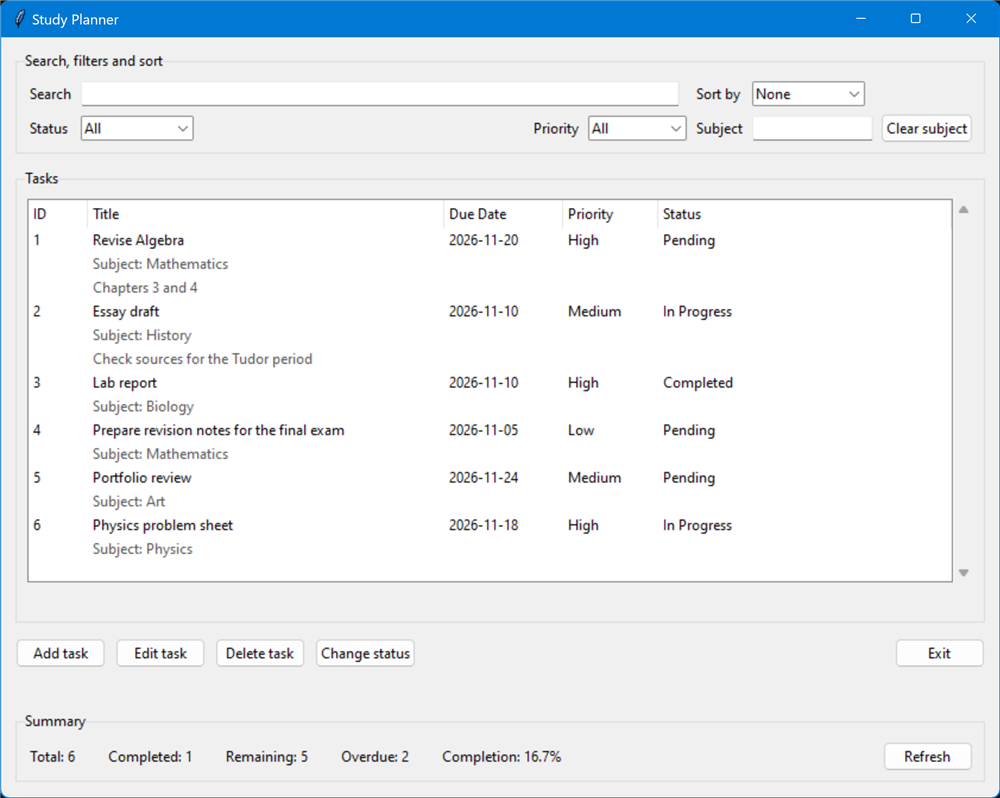
\includegraphics[width=0.85\textwidth]{gui-main.png}
\caption{The GUI version with demonstration data.}
\label{fig:gui}
\end{figure}

% ---------------------------------------------------------------------------
\section{Testing}
\label{sec:testing}

\subsection{Approach}
Tests use the standard \code{unittest} module \parencite{python-unittest}
and run from the repository root
with \code{python -m unittest discover -s tests}. They are written per module:
validation, storage, core operations, the text version (scripted input and
captured output) and the GUI (a hidden Tk window, destroyed after each test).
Data files are created only in temporary folders, and the date is fixed in
date-dependent tests. Per-rule variants are tested once on the core, with
representative cases through each interface.

\subsection{Test plan and cases}
The test plan lists 304 test cases, each with its requirement, kind, input and
exact expected result: 136 normal, 77 boundary and 91 invalid cases
(Table~\ref{tab:plan}). Boundary cases include the 29 February in leap and
non-leap years, a task due exactly today (not overdue), a 30-character title
that just fits its column and 1 completed task out of 16 for the half-up
rounding. Invalid cases include 38 invalid data files, each checked to be
left byte-for-byte unchanged, and failed saves produced by a read-only file.

\begin{table}[ht]
\centering
\small
\begin{tabular}{@{}lrl@{}}
\toprule
Area & Cases & Test IDs \\
\midrule
FR5 validation (core) & 59 & V1--V59 \\
FR6 persistence (storage, core, text version) & 34 & S1--S34 \\
FR1--FR4 task operations (core and text version) & 47 & A, E, D, C \\
FR7--FR10 search, filters, sort, summary & 74 & SR, F, SO, SU \\
FR11 list view and messages & 19 & VW, M \\
GUI version & 71 & G1--G71 \\
\midrule
Total & 304 & \\
\bottomrule
\end{tabular}
\caption{Test cases by area.}
\label{tab:plan}
\end{table}

\subsection{Results}
All 317 automated tests pass (Python 3.12.5, Windows 11, 13 November 2026).
The suite was run on a clean copy of every development stage, and its size
grew with the features: 92 tests for validation and storage, 124 with the
task operations, 164 with the text version, 246 with search, filters, sort
and summary, and 317 with the GUI. The same tests also pass in a fresh virtual
environment with no packages installed. A verification matrix records, for
every requirement, the passing tests in each version.

Further checks support the results:
\begin{itemize}
  \item \textbf{Coverage.} \code{coverage.py} \parencite{coveragepy}
        measures 97\% statement and branch
        coverage of the source code. The uncovered lines are mainly the
        programs' start-up code, which was checked by launching both versions.
  \item \textbf{Deliberate faults.} During development, faults were inserted
        into the code one at a time (for example an unstable merge, a missing
        \code{casefold()}, a task due today counted as overdue, or a closed
        delete dialog that still deleted). Each fault had to make at least one
        test fail; where one did not, a test was added.
  \item \textbf{Performance (NFR6).} On 500 generated tasks, a search took
        0.35--0.46\,ms and a merge sort 0.80--0.88\,ms per call (fastest of
        7 repeats of 50 calls, measured with \code{timeit}
        \parencite{python-timeit}).
  \item \textbf{Manual GUI checks.} The GUI was launched with demonstration
        data and its main workflows were checked on the real event loop,
        including an add form showing the core's validation error and the
        unsaved-changes dialog.
\end{itemize}

% ---------------------------------------------------------------------------
\section{Evaluation}

\subsection{Against the requirements}
All eleven functional and nine non-functional requirements are met, and every
one of the 77 acceptance criteria has at least one passing test. The two
versions offer the same functionality: the GUI tests repeat the acceptance
criteria that apply to a graphical interface, and the criteria that do not
apply (typing an invalid task ID or status where the GUI only offers valid
choices) are recorded as not applicable rather than skipped. The shared core
proved its value when the GUI was built: it needed no new rules, and the core
gained no interface-specific code.

\subsection{Limitations}
\begin{itemize}
  \item With a search active, the text version can act on a hidden task by
        typing its ID, while the GUI can act only on visible rows; this
        difference is deliberate but must be learnt by the user.
  \item The exit prompt cannot appear if the program is ended forcibly, for
        example with Ctrl+C or a system shutdown.
  \item Column widths in the text version count characters, so wide (for
        example East Asian) characters can misalign the table.
  \item In the GUI, long descriptions are shortened visually by the fixed
        column width; the full text is shown in the edit form.
  \item When the GUI is started without a console (\code{pythonw}), error
        details written to standard error are not visible.
  \item The planner is single-user and stores one local file; there is no
        backup or synchronisation.
  \item The GUI tests need a display and are skipped, with a reason, where
        none exists.
\end{itemize}

\subsection{Future improvements}
Possible extensions are reminders for tasks due soon, an undo for the last
change, export of the task list to CSV, keyboard shortcuts in the GUI and a
measured performance threshold for larger task lists.

\yourwords{optional: a short critical reflection on what worked well and what
you would do differently. Describe only your own experience.}

% ---------------------------------------------------------------------------
\section{Conclusion}
The Study Planner meets its aims: students can add, edit, delete and track
study tasks, find them through search, filters and a stable merge sort, and
see their progress, in a text-based and a graphical version with the same
behaviour. Keeping every rule in one core module made the two versions
consistent and the code testable, and strict loading with safe saving keeps
the user's data intact even when saving fails. A traceable test plan of 304
cases and 317 passing automated tests provide the evidence that the
requirements are met.

% ---------------------------------------------------------------------------
\section*{GenAI acknowledgement}
\addcontentsline{toc}{section}{GenAI acknowledgement}
\yourwords{check and rewrite this draft so that it describes your use
exactly.} I used Claude (Anthropic), through the Claude Code tool, during this
project. It wrote most of the Python source code and the automated tests under
my direction, drafted parts of the requirements, design and test
documentation and of this report for my review, ran the tests and checks, and
carried out Git and GitHub operations. I chose the topic, decided the
requirements and design choices, reviewed and corrected the outputs, and I am
responsible for the submitted work.

\clearpage
\printbibliography[heading=bibintoc]

\clearpage
\appendix
\section{How to install and run both applications}

\paragraph{Requirements.} Python 3.12 with Tkinter, which is included with the
standard Python installers for Windows and macOS. No other packages are
needed, so there is no \code{requirements.txt}. To check that Tkinter works,
run \code{python -m tkinter}; a small window should open.

\paragraph{Installation.} Unzip the submission, or clone the repository, and
open a terminal in the project folder (the folder that contains \code{src}
and \code{tests}).

\paragraph{Running the text-based version.}
\begin{lstlisting}[numbers=none]
python src/cli.py
\end{lstlisting}
Choose options by number from the menu; \code{0} exits.

\paragraph{Running the GUI version.}
\begin{lstlisting}[numbers=none]
python src/gui.py
\end{lstlisting}
Select a task in the list, then use the buttons; double-clicking a task opens
it for editing. Start the GUI from a terminal to see error details.

\paragraph{Running the tests.}
\begin{lstlisting}[numbers=none]
python -m unittest discover -s tests
\end{lstlisting}

\paragraph{Data file.} Tasks are saved in
\code{\textasciitilde/.study\_planner/tasks.json} in the user's home folder. The
file and its folder are created by the first successful save.

\end{document}
